\documentclass{beamer}
\usetheme{metropolis} 

\usepackage{filecontents}
\usepackage{natbib}
%\usepackage{luabibentry}
%\setupbibentry{\jobname}
\usepackage{booktabs}
\usepackage[scale=2]{ccicons}
\usepackage{adjustbox}
%\usepackage{media9}
\usepackage{bibentry}
\usepackage{hyperref}
%\usepackage{movie15}
\usepackage{enumerate}
\usepackage{amsmath,color,float,graphicx}
\usepackage{multimedia}
\usepackage{animate,bm}
\usepackage{subcaption}
\usepackage{empheq}
\usepackage{cancel}

\global\long\def\V#1{\boldsymbol{#1}}
\global\long\def\M#1{\boldsymbol{#1}}
\global\long\def\Set#1{\mathbb{#1}}


\global\long\def\D#1{\Delta#1}
\global\long\def\d#1{\delta#1}


\global\long\def\norm#1{\left\Vert #1\right\Vert }
\global\long\def\abs#1{\left|#1\right|}


\global\long\def\grad{\M{\nabla}}
\global\long\def\avv#1{\langle#1\rangle}
\global\long\def\av#1{\left\langle #1\right\rangle }


\global\long\def\P{\mathcal{P}}


\global\long\def\ki{k}
\global\long\def\wi{\omega}


\global\long\def\slip{\breve{\V u}}


\global\long\def\bu{\V u}
\global\long\def\bv{\V v}
\global\long\def\br{\V r}


\global\long\def\sM#1{\M{\mathcal{#1}}}
\global\long\def\Mob{\sM M}
\global\long\def\J{\sM J}
\global\long\def\S{\sM S}
\global\long\def\L{\sM L}


\global\long\def\N{\sM N}
\global\long\def\K{\sM K}
\global\long\def\slipN{\breve{\N}}

\global\long\def\rhat{\hat{\V{r}}}
\global\long\def\mhat{\bar{\V{m}}}

\global\long\def\eqd{\overset{d}{=}}


\global\long\def\aN{\widetilde{\N}}
\global\long\def\aK{\widetilde{\K}}
\global\long\def\aMob{\widetilde{\Mob}}


\global\long\def\epsN{\overline{\N}}


\global\long\def\slipW{\breve{\V W}}
\global\long\def\rot{\M{\Psi}}
\global\long\def\Rot{\M{\Xi}}


% \usepackage{epstopdf}
% \epstopdfDeclareGraphicsRule{.tif}{png}{.png}{convert #1 \OutputFile}
% \AppendGraphicsExtensions{.tif}



\newcommand*\widefbox[1]{\fbox{\hspace{1.5em}#1\hspace{1.5em}}}
\providecommand{\noop}[2]{#2}
          % Use metropolis theme
\title{Hydrodynamics of magnetic chains, and flexible fibres with a twist}
\date{\today}
\author{Brennan Sprinkle}
\begin{document}
  \maketitle
  
\section{Outline}
\begin{frame}
\frametitle{Orders of business}
\begin{enumerate}
\item Problem set up 
\item The model/method we used
\item Towards a new method
\end{enumerate}
\end{frame}  
  
\section{Colloidal Chains}

{%<--- Start local changes
\setbeamertemplate{navigation symbols}{}
\usebackgroundtemplate{%
  \vbox to \paperheight{\vfil\hbox to \paperwidth{\hfil\includegraphics[width=\paperwidth]{./Intro_Image/Chain_Cartoon_flat_1.png}\hfil}\vfil}
}
\begin{frame}[plain]
\end{frame}
}%<---- Finish local changes


{%<--- Start local changes
\setbeamertemplate{navigation symbols}{}
\usebackgroundtemplate{%
  \vbox to \paperheight{\vfil\hbox to \paperwidth{\hfil\includegraphics[width=\paperwidth]{./Intro_Image/Chain_Cartoon_flat_2.png}\hfil}\vfil}
}
\begin{frame}[plain]
\end{frame}
}%<---- Finish local changes

{%<--- Start local changes
\setbeamertemplate{navigation symbols}{}
\usebackgroundtemplate{%
  \vbox to \paperheight{\vfil\hbox to \paperwidth{\hfil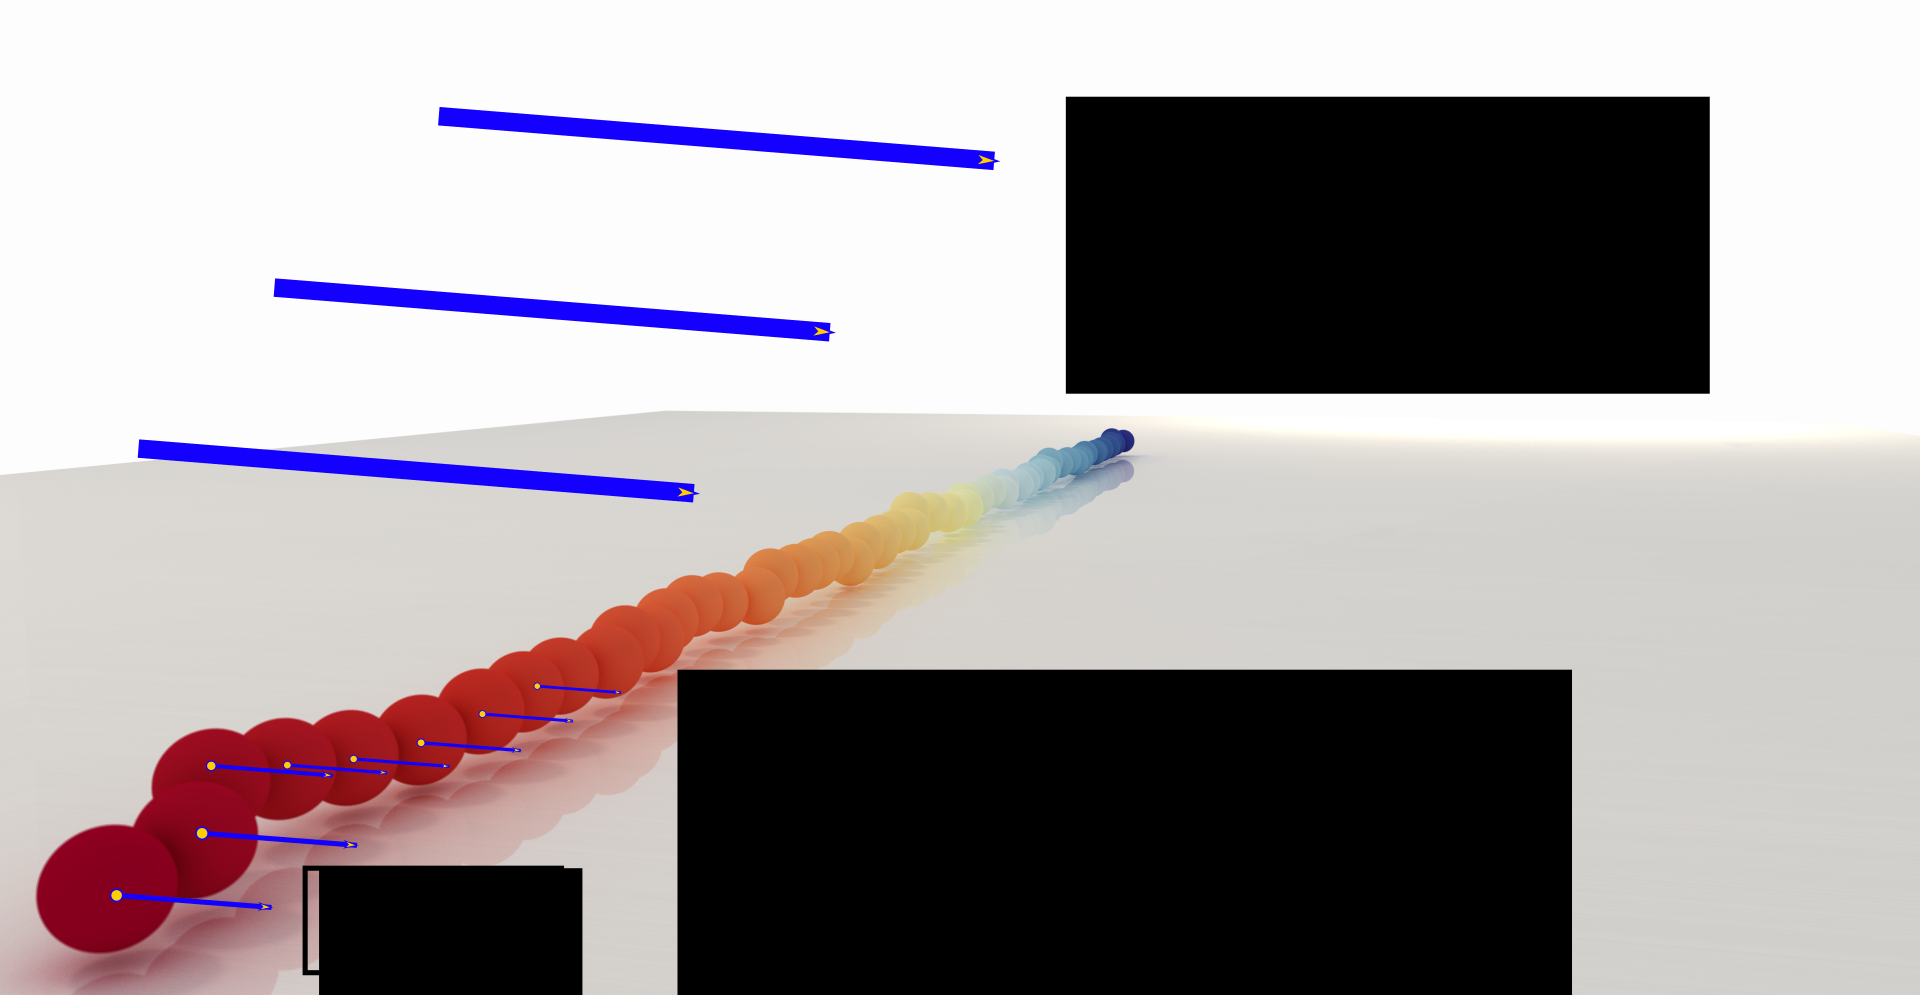
\includegraphics[width=\paperwidth]{./Intro_Image/Chain_Cartoon_flat_3.png}\hfil}\vfil}
}
\begin{frame}[plain]
\end{frame}
}%<---- Finish local changes


{%<--- Start local changes
\setbeamertemplate{navigation symbols}{}
\usebackgroundtemplate{%
  \vbox to \paperheight{\vfil\hbox to \paperwidth{\hfil\includegraphics[width=\paperwidth]{./Intro_Image/Chain_Cartoon_4.png}\hfil}\vfil}
}
\begin{frame}[plain]
\end{frame}
}%<---- Finish local changes


\section{Experiments}

\section{Simulation}


\section{Magnetic Model}
\begin{frame}
\frametitle{Magnetic Force}
Superparamagnetic particles (almost) instantaneously develop a magnetic moment $\mhat$ aligned with the applied magnetic field $\V{B}(t)$ so that 
\[
\mhat \propto \V{B}(t) = B_{\text{DC}} \V{\hat{x}} + B_{\text{AC}} \sin\left( 2 \pi (50 \text{Hz}) t \right) \V{\hat{y}} + B_{\text{AC}} \sin\left( 2 \pi (50 \text{Hz}) t \right) \V{\hat{z}}.
\]
In a chain of $N$ beads, the magnetic force on bead $i$ due to the interaction with bead $j$ is 
\begin{equation}
\V{f}^{\text{mag}}_{i,j} = \frac{F_0}{(r_{i,j}/a)^{4}} \left( 2 \left( \mhat \cdot \rhat_{i,j} \right) \mhat - \left( 5 \left( \mhat \cdot \rhat_{i,j} \right)^2 - 1 \right) \rhat_{i,j} \right),
\end{equation}
where $F_0 = 2.6 \times 10^{-12}$N is the strength of the magnetic interactions. 
\end{frame}

\begin{frame}
\frametitle{Magic Angle}
We can define the `angle' $\beta$ of the magnetic field 
\[
\V{B}(t) = B_{\text{DC}} \V{\hat{x}} + B_{\text{AC}} \sin\left( 2 \pi (50 \text{Hz}) t \right) \V{\hat{y}} + B_{\text{AC}} \sin\left( 2 \pi (50 \text{Hz}) t \right) \V{\hat{z}}.
\]
as
\[
\beta = \arctan \left( \frac{B_{\text{AC}}}{B_{\text{DC}}} \right).
\]
And it was observed in experiments that the chains formed a helix shape for
\[
\beta \approx 55^{\circ},
\]
where stretching from $B_{\text{DC}}$, and twirling from $B_{\text{AC}}$ are in balance.
\end{frame}

\section{Chain Model}

\begin{frame}
\frametitle{Requirements}
\begin{itemize}
\item We maintain inextensibility between the centers of neighboring beads $\V{x}_i$ and $\V{x}_{i+1}$
\item The particles in the chain are bonded together so they shouldn't `twist' much relative to each other. 
\item The chain should be able to bend with modulus $\kappa_b$
\end{itemize}    
\end{frame}

\begin{frame}
\frametitle{Heterogeneity in Bending}
The chains in experiments clearly have a preferred chirality from a heterogeneity built into them during synthesis. We model this as a linearly decaying bending stiffness
\[
 \kappa_b\left(s\right) = \kappa_b^{\text{const.}} \frac{3 + 2 (i/N) }{5} 
\]
\end{frame}

%\begin{frame}
%\frametitle{Forces and Torques}
%Internal forces on bead $i$ of the chain are computed by varying the internal energy $U_{\text{chain}}$ with respect to the center-line $\V{x}_i$
%\[
%\V{f}^{\text{chain}}_i = \delta_{\V{x}_i} U_{\text{chain}} = \delta_{\V{x}_i} \left( U_{\text{spring}} + U_{\text{bend}} \right).
%\]
%The total forces on bead $i$ in the chain are
%\begin{align}
%\V{f}_i = \V{f}^{\text{chain}}_i + \displaystyle \sum_{j > i} \V{f}^{\text{mag}}_{i,j}. 
%\end{align}
%Torque on the particles is not important for now
%%\[
%%\V{T}_i &= \displaystyle \sum_{j} \V{r}_{i,j} \times \V{f}_j
%%\]
%\end{frame}

\section{ Kirchhoff Rods}

\begin{frame}
\frametitle{Particle orientation}
At each bead, we affix an othonormal triad 
\[
\M{Q}_i = [\V{D}^{1}_i, \V{D}^{2}_i, \V{D}^{3}_i],
\]
and constrain $\V{D}^{3}_i = \left( \V{x}_{i+1} - \V{x}_{i} \right) \approx \V{x}^{'}(s) = \V{t}(s)$. 
\begin{figure}
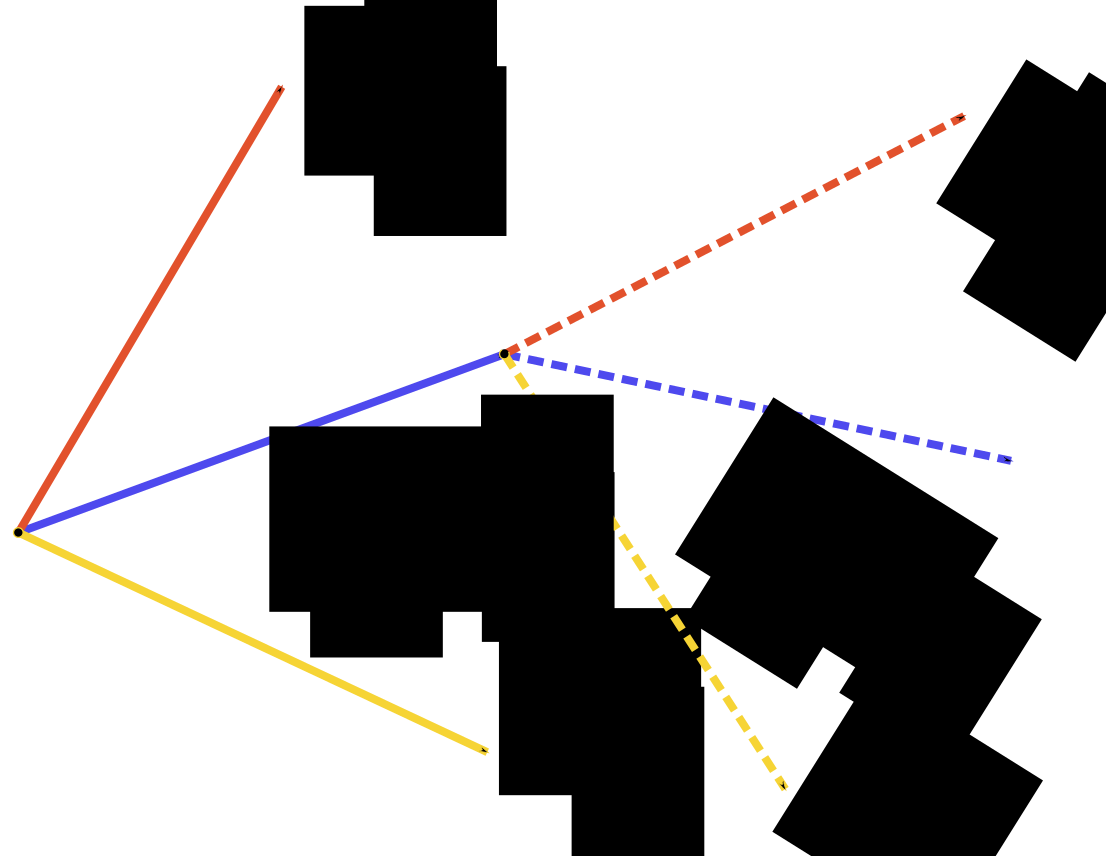
\includegraphics[height=0.6\textheight,width=0.5\textwidth]{./Cartoons/Frames.pdf}
\end{figure}
\end{frame}

\begin{frame}
\frametitle{Kirchhoff Rods}
\begin{alertblock}{Assume the frames at two neighboring beads only differ by a small rotation}
Let $s$ be arclength along the chain.
\[
\partial_{s} \M{Q} = \M{\Omega} \times \M{Q}
\]
Using \[\V{D}^{1} = \V{D}^{2} \times \V{D}^{3}, \ \cdots\] we get
\begin{align}
\M{\Omega} &=  \Omega_1 \V{D}^{1} +  \Omega_2 \V{D}^{2} +  \Omega_3 \V{D}^{3} \\ 
&= \left( \V{D}^{2}_{s} \cdot \V{D}^{3} \right) \V{D}^{1} +  \left( \V{D}^{3}_{s} \cdot \V{D}^{2} \right) \V{D}^{2} +  \left( \V{D}^{1}_{s} \cdot \V{D}^{2} \right) \V{D}^{3}
\end{align}
and discretize $\V{D}^{k}_{s} \approx \V{D}^{k}_{i+1/2} - \V{D}^{k}_{i-1/2}$
\end{alertblock}
\end{frame}


\begin{frame}
\frametitle{Penalty Method}
Lim and Peskin give forces and torques on the particles as
\alert<1->{
\begin{align}
- \V{f}^{ch} &= \overbrace{\partial_{s} \V{\Lambda}}^{(1)} \\
- \V{\tau}^{ch} &= \partial_{s} \underbrace{\V{M}(s)}_{(2)} + \underbrace{\left( \partial_{s} \V{x} \right) \times \V{\Lambda}}_{(3)}
\end{align}
}
where $\V{\Lambda}$ enforces that the triad be orthogonal and that $\V{D}^{3}_i = \left( \V{x}_{i+1} - \V{x}_{i} \right) \approx \partial_{s} \V{x} = \V{t}(s)$.
\begin{align}
 \V{\Lambda} &= \Lambda_1 \V{D}^{1} +  \Lambda_2 \V{D}^{2} +  \Lambda_3 \V{D}^{3} \\
 &= \underbrace{\kappa_S \left( \V{D}^{1} \cdot \V{t} \right) \V{D}^{1} +  \kappa_S \left( \V{D}^{2} \cdot \V{t} \right) \V{D}^{2}}_{(a)} +  \underbrace{\kappa_S \left( \V{D}^{3} \cdot \V{t} -1 \right) \V{D}^{3}}_{(b)}
\end{align}
And
\[
\V{M}(s) = \left( \kappa_b \left[\Omega_1 \V{D}^{1} +  \Omega_2 \V{D}^{2} \right] +  \kappa_T \Omega_3 \V{D}^{3} \right)
\]
 
\end{frame}

\begin{frame}
\frametitle{Force and Torque on the Chain}
The force and torque on bead $i$ in the chain is 
\begin{align}
\V{f}_{i} &= \V{f}_{i}^{ch} + \displaystyle \sum_{j > i} \V{f}^{\text{mag}}_{i,j} \\
\V{\tau}_{i} &= \V{\tau}_{i}^{ch} + \displaystyle \sum_{j > i} \V{\tau}^{\text{mag}}_{i,j}
\end{align}
 
\end{frame}

\section{hydrodynamics}

\begin{frame}
\frametitle{Equation of motion}

Chains are small enough that steady Stokes equations govern hydrodynamics. Linearity of Stokes means that we can write 
\begin{align}
 \begin{bmatrix} \V{U}_1 \\ \vdots \\ \V{U}_N \end{bmatrix} &=  \N \left( \V{x}_1,\cdots,\V{x}_n \right) \cdot \begin{bmatrix} \V{F}_1 \\ \vdots \\ \V{F}_N \end{bmatrix}, \ \ \ \,\V{U}_i = \begin{bmatrix} \V{u}_i \\ \V{\omega}_i \end{bmatrix}, \ \V{F}_i = \begin{bmatrix} \V{f}_i \\ \V{\tau}_i \end{bmatrix}
\end{align}
\vspace{-0.5cm}
\begin{alertblock}{Mobility}
\begin{itemize}
\item $\N \left( \V{x}_1,\cdots,\V{x}_n \right)$ is a 'Friction' or 'Mobility' operator that depends of the configuration of every particle in the chain and the geometry of the domain (e.g. bottom wall)
\end{itemize}
\end{alertblock}
\begin{exampleblock}{Update position}
we integrate $\V{x}_i, \M{Q}_i$ according to 
\vspace{-0.25cm}
\begin{align}
 \partial_{t} \V{x}_i &=  \V{u}_i, \\
 \partial_{t} \M{Q}_i &= \V{\omega}_i \times \M{Q}_i,
 \vspace{-0.25cm}
\end{align}
\end{exampleblock}

\end{frame}

\begin{frame}
\frametitle{Details in Hydrodynamics}
\begin{itemize}
\item Chains are small enough that hydrodynamics also must include terms which capture thermal fluctuations from the fluid. These are included but we won't really discuss them.
\item Since the beads are so close together, we include lubrication corrections in the mobility
\[
\bar{\N} = \left( \N^{-1} - \N_{\text{close particles}}^{-1} + \left(\N_{\text{close particles}}^{\text{asymptotics}}\right)^{-1} \right)^{-1}
\]
and steric repulsion to keep the beads from overlapping
\end{itemize}
\end{frame}


\section{Comparison With experiments}

\section{Another Way}
\begin{frame}
\frametitle{Problems With Kirchhoff}
\begin{enumerate}
\item Unnecessary degrees of freedom (position and orientation of every particle in the chain)
\item Penalty formulation imposes a potentially large time step restriction 
\end{enumerate}
\end{frame}

\begin{frame}
\frametitle{New Coordinates}
We should be able to model chains using only their unit tangent vectors $\V{t}_i$ and a scalar `twist' $\theta_i$ off of a reference axis (more on $\theta_i$ in coming slides). Given a set of unit tangent vectors 
\[
\left\{ \V{t}_1,  \V{t}_2, \cdots ,  \V{t}_N \right\}
\]
we can find 
\[
\V{x}_{i} = \V{x}_{0} + \displaystyle \sum_{j = 1}^{i-1} \V{t}_i \approx \V{x}_{0} + \displaystyle \int_{0}^{s} \V{t}(s') ds'
\]
as a map from 
\[
\V{t} \in S^{2} \rightarrow \V{x} \in \mathbb{R}^{3}
\]
\end{frame}

\begin{frame}
\frametitle{New Coordinates}
\begin{figure}
\includegraphics[width=1\textwidth]{./Cartoons/Tangent_Sphere.png}
\end{figure}
\end{frame}



\begin{frame}
\frametitle{New Coordinates}
For a straight chain pointing \emph{into} the page, we can define $\V{z}$ as a reference axis and measure the local twist $\theta_i$ off of this axis. 
\begin{figure}
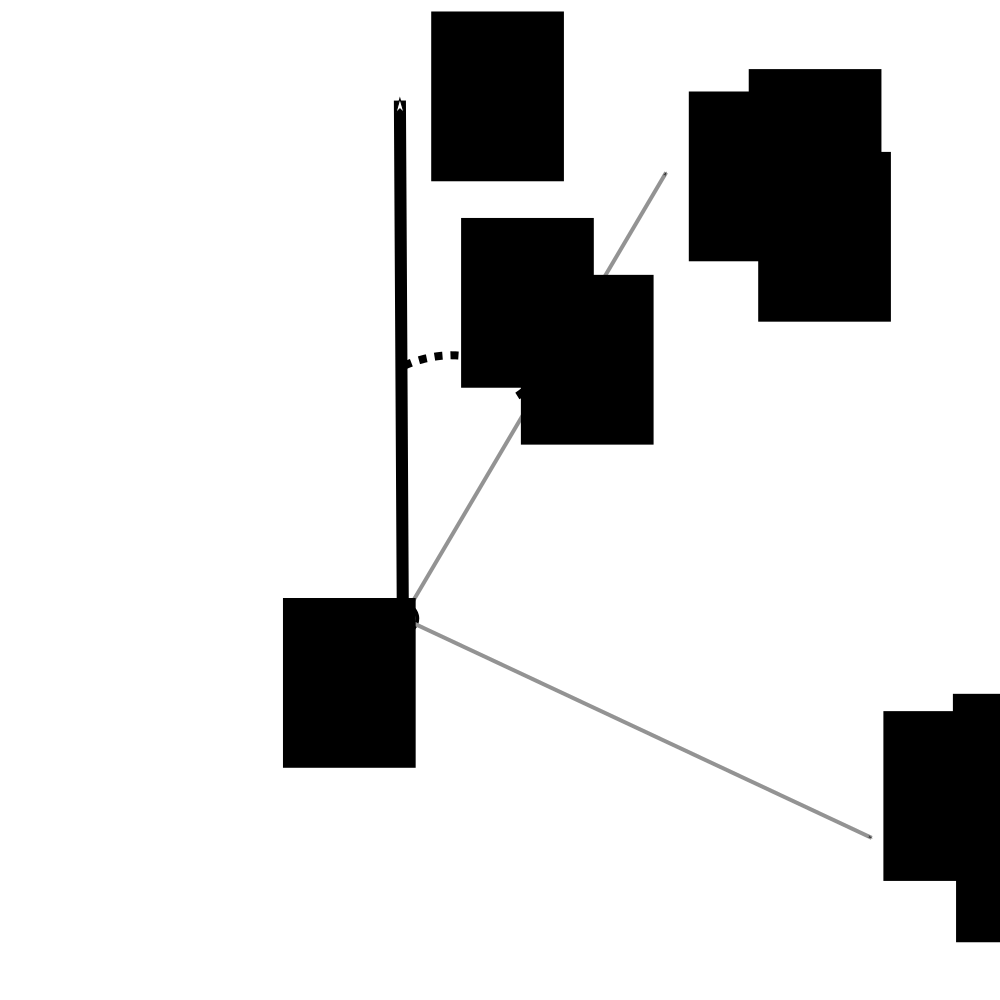
\includegraphics[height=0.6\textheight,width=0.5\textwidth]{./Cartoons/Theta.pdf}
\end{figure}
\alert{But what about a curved chain?}
\end{frame}

\begin{frame}
\frametitle{Bishop Frame}
\begin{alertblock}{Recall}
\[
\partial_{s} \V{t} = \M{\Omega} \times \V{t}
\]
\end{alertblock}
We can write 
\[
\M{\Omega} = m(s) \V{t} + \V{t} \times  \V{t}_{s}
\]
where $m(s) = \left( \V{D}^{1}_{s} \right) \cdot \V{D}^{2}$ is the `rate of twist'.
\end{frame} 
  
\begin{frame}
\frametitle{Bishop Frame}

The material frame 
\[
\M{Q}(s) = [\V{D}^{1}(s), \V{D}^{2}(s), \V{D}^{3}(s)],
\]
is to be determined by the physics of the problem. 

But we can define a new `intrinsic frame' (Bishop frame) so that the rate of twist vanishes.
\begin{align}
\M{B}(s) &= [\V{t}(s), \V{u}(s), \V{v}(s)] \hspace{1cm} \text{   such that   } \\
m_{B}(s) &= \V{u}_{s} \cdot \V{v} = 0
\end{align}
and
\[
\M{\Omega}_{B} = \cancel{m_B(s) \V{t}} + \V{t} \times  \V{t}_{s}
\]
\end{frame} 
  
\begin{frame}
\frametitle{Bishop Frame}
In the Bishop frame 
\[
\partial_{s} \V{u} = \left(\V{t} \times \V{t}_s \right) \times \V{u} \text{   (no twist)   }
\] 
which is integrable as
\[
\V{u}(s) = \underbrace{\exp \left( s \ \left[ \V{t} \times \V{t}_s \right]_{\times} \right)}_{\M{P}}  \V{u}(0), \ \ \ \ \  \V{v}(s) = \V{t}(s) \times \V{u}(s)
\] 
where $\M{P}$ is a rotation matrix such that $\V{t}(s + ds) =  \M{P} \cdot \V{t}(s)$, or a \emph{parallel transport map}.
\end{frame} 

\begin{frame}
\frametitle{Bishop Frame}
Given $\V{t}(s)$ and $\V{u}(0),\V{v}(0)$ (which are arbitrary), the Bishop frame is completely determined. We use the bishop frame as a reference frame for measuring $\theta$.
\begin{figure}
\includegraphics[height=0.6\textheight,width=0.5\textwidth]{./Cartoons/Bishop.pdf}
\end{figure}
\end{frame} 

\begin{frame}
\frametitle{New Coordinates}
\begin{figure}
\includegraphics[width=1\textwidth]{./Cartoons/Bishop_Sphere.png}
\end{figure}
\end{frame}

\begin{frame}
\frametitle{Bishop Frame}
From the Bishop frame and $\theta(s)$, we compute the material frame as
\begin{align}
\V{D}^{1} &= \cos (\theta) \V{u} + \sin(\theta) \V{v} \\
\V{D}^{2} &= -\sin (\theta) \V{u} + \cos(\theta) \V{v}
\end{align}
Hence
\[
m(s) = \left( \V{D}^{1}_{s} \right) \cdot \V{D}^{2} = \theta_s
\]
and
\begin{align}
\M{\Omega} &= \underbrace{\theta_s}_{\Omega_3} \V{t} + \underbrace{\V{t} \times  \V{t}_{s}}_{\Omega_1 \V{D}^{1} +  \Omega_2 \V{D}^{2}}
\end{align}
\end{frame}

\begin{frame}
\frametitle{Energy}
\alert<1->{
\begin{align*}
\M{\Omega} &= \underbrace{\theta_s}_{\Omega_3} \V{t} + \underbrace{\V{t} \times  \V{t}_{s}}_{\Omega_1 \V{D}^{1} +  \Omega_2 \V{D}^{2}}
\end{align*}
}
The energy functional for a constrained ($\V{x}_s = \V{t}$) Kirchhoff rod is 
\begin{align}
\M{E} &= \frac{1}{2} \displaystyle \int_{0}^{L} \kappa_b \left(  \Omega_1^{2} +  \Omega_2^{2}  \right) +  \kappa_T \Omega_3^{2}  + \overbrace{\Lambda(s) }^{\text{Lagrange mult.}}  ds \\
&= \frac{1}{2} \displaystyle \int_{0}^{L} \kappa_b \left(  \alert{|| \V{t} \times  \V{t}_{s} ||^2} \right) +  \kappa_T \left(\alert{\theta_s} \right)^{2}  + \Lambda(s)  \\
&= \frac{1}{2} \displaystyle \int_{0}^{L} \kappa_b \underbrace{\left(  \alert{|| \V{t}_{s} ||^2} \right)}_{\text{Euler Beam}} +  \kappa_T \left(\alert{\theta_s} \right)^{2}  + \Lambda(s) 
\end{align}

\end{frame}

\begin{frame}
\frametitle{Variation of the energy}
We get the torque on out particles from $\M{E}$ easily by varying theta
\[
\V{\tau} = -\frac{\delta}{\delta \theta} \M{E} = -\kappa_T \theta_{ss}
\]
\begin{alertblock}{The force is a bit more nuanced.}
 We vary the center-line $\V{x}(s) \leftarrow \V{x}(s) + \delta \V{x}(s)$ and compute
\[
\V{f} = -\frac{\delta \M{E} }{\delta \V{x}}   -\frac{\delta \M{E}}{\delta \theta_s} \frac{\delta \theta_s}{\delta \V{x}} 
\]
\end{alertblock}
\end{frame}

\begin{frame}
\frametitle{Variation of the energy}
The quantity 
\alert<1->{
\[
\frac{\delta \theta_s}{\delta \V{x}} 
\]
}
is tantamount to the variation of the Bishop frame along centerline
\[
\frac{\delta \theta_s}{\delta \V{x}} = \V{u}_s \sphericalangle \frac{\delta \V{u}_s}{\delta \V{x}}
\]
\end{frame} 

\begin{frame}
\frametitle{Holonomy}
\begin{figure}
\includegraphics[height=0.6\textheight,width=0.5\textwidth]{./Holonomy/Holonomy_Anotated}
\end{figure}
\[
\frac{\delta \theta_s}{\delta \V{x}} = \V{u} \angle \delta \V{u} \approx ||\V{t}_{s} \times \delta \V{x}_{s} || = \left( \V{t} \times \V{t}_{s} \right) \cdot \delta \V{x}_{s} ds 
\]
\end{frame} 

\begin{frame}
\frametitle{Variation of the energy}
\begin{align}
\V{\tau} &= -\frac{\delta}{\delta \theta} \M{E} = -\kappa_T \theta_{ss} \\
\V{f} &= -\frac{\delta \M{E} }{\delta \V{x}}   -\frac{\delta \M{E}}{\delta \theta_s} \frac{\delta \theta_s}{\delta \V{x}} \\
&= \kappa_b \V{x}_{ssss}   - \kappa_T \big( \underbrace{\theta_{s}}_{\text{from } \frac{\delta \M{E}}{\delta \theta_s}} \overbrace{\left(\V{t} \times \V{t}_{s}\right)}^{\text{from } \frac{\delta \theta_s}{\delta \V{x}}}  \big)_{s} + \left( \Lambda \V{t} \right)_s
\end{align}

\end{frame}


\begin{frame}
\frametitle{Next Steps}
\begin{alertblock}{Open question:}
How to do hydrodynamics with constrained chains and twist. 
\end{alertblock}

\end{frame}


\end{document}